\documentclass[]{article}
\usepackage{lmodern}
\usepackage{amssymb,amsmath}
\usepackage{ifxetex,ifluatex}
\usepackage{fixltx2e} % provides \textsubscript
\ifnum 0\ifxetex 1\fi\ifluatex 1\fi=0 % if pdftex
  \usepackage[T1]{fontenc}
  \usepackage[utf8]{inputenc}
\else % if luatex or xelatex
  \ifxetex
    \usepackage{mathspec}
  \else
    \usepackage{fontspec}
  \fi
  \defaultfontfeatures{Ligatures=TeX,Scale=MatchLowercase}
\fi
% use upquote if available, for straight quotes in verbatim environments
\IfFileExists{upquote.sty}{\usepackage{upquote}}{}
% use microtype if available
\IfFileExists{microtype.sty}{%
\usepackage{microtype}
\UseMicrotypeSet[protrusion]{basicmath} % disable protrusion for tt fonts
}{}
\usepackage[margin=1in]{geometry}
\usepackage{hyperref}
\hypersetup{unicode=true,
            pdftitle={Machine Learning in R},
            pdfauthor={Jim Gruman},
            pdfborder={0 0 0},
            breaklinks=true}
\urlstyle{same}  % don't use monospace font for urls
\usepackage{color}
\usepackage{fancyvrb}
\newcommand{\VerbBar}{|}
\newcommand{\VERB}{\Verb[commandchars=\\\{\}]}
\DefineVerbatimEnvironment{Highlighting}{Verbatim}{commandchars=\\\{\}}
% Add ',fontsize=\small' for more characters per line
\usepackage{framed}
\definecolor{shadecolor}{RGB}{248,248,248}
\newenvironment{Shaded}{\begin{snugshade}}{\end{snugshade}}
\newcommand{\AlertTok}[1]{\textcolor[rgb]{0.94,0.16,0.16}{#1}}
\newcommand{\AnnotationTok}[1]{\textcolor[rgb]{0.56,0.35,0.01}{\textbf{\textit{#1}}}}
\newcommand{\AttributeTok}[1]{\textcolor[rgb]{0.77,0.63,0.00}{#1}}
\newcommand{\BaseNTok}[1]{\textcolor[rgb]{0.00,0.00,0.81}{#1}}
\newcommand{\BuiltInTok}[1]{#1}
\newcommand{\CharTok}[1]{\textcolor[rgb]{0.31,0.60,0.02}{#1}}
\newcommand{\CommentTok}[1]{\textcolor[rgb]{0.56,0.35,0.01}{\textit{#1}}}
\newcommand{\CommentVarTok}[1]{\textcolor[rgb]{0.56,0.35,0.01}{\textbf{\textit{#1}}}}
\newcommand{\ConstantTok}[1]{\textcolor[rgb]{0.00,0.00,0.00}{#1}}
\newcommand{\ControlFlowTok}[1]{\textcolor[rgb]{0.13,0.29,0.53}{\textbf{#1}}}
\newcommand{\DataTypeTok}[1]{\textcolor[rgb]{0.13,0.29,0.53}{#1}}
\newcommand{\DecValTok}[1]{\textcolor[rgb]{0.00,0.00,0.81}{#1}}
\newcommand{\DocumentationTok}[1]{\textcolor[rgb]{0.56,0.35,0.01}{\textbf{\textit{#1}}}}
\newcommand{\ErrorTok}[1]{\textcolor[rgb]{0.64,0.00,0.00}{\textbf{#1}}}
\newcommand{\ExtensionTok}[1]{#1}
\newcommand{\FloatTok}[1]{\textcolor[rgb]{0.00,0.00,0.81}{#1}}
\newcommand{\FunctionTok}[1]{\textcolor[rgb]{0.00,0.00,0.00}{#1}}
\newcommand{\ImportTok}[1]{#1}
\newcommand{\InformationTok}[1]{\textcolor[rgb]{0.56,0.35,0.01}{\textbf{\textit{#1}}}}
\newcommand{\KeywordTok}[1]{\textcolor[rgb]{0.13,0.29,0.53}{\textbf{#1}}}
\newcommand{\NormalTok}[1]{#1}
\newcommand{\OperatorTok}[1]{\textcolor[rgb]{0.81,0.36,0.00}{\textbf{#1}}}
\newcommand{\OtherTok}[1]{\textcolor[rgb]{0.56,0.35,0.01}{#1}}
\newcommand{\PreprocessorTok}[1]{\textcolor[rgb]{0.56,0.35,0.01}{\textit{#1}}}
\newcommand{\RegionMarkerTok}[1]{#1}
\newcommand{\SpecialCharTok}[1]{\textcolor[rgb]{0.00,0.00,0.00}{#1}}
\newcommand{\SpecialStringTok}[1]{\textcolor[rgb]{0.31,0.60,0.02}{#1}}
\newcommand{\StringTok}[1]{\textcolor[rgb]{0.31,0.60,0.02}{#1}}
\newcommand{\VariableTok}[1]{\textcolor[rgb]{0.00,0.00,0.00}{#1}}
\newcommand{\VerbatimStringTok}[1]{\textcolor[rgb]{0.31,0.60,0.02}{#1}}
\newcommand{\WarningTok}[1]{\textcolor[rgb]{0.56,0.35,0.01}{\textbf{\textit{#1}}}}
\usepackage{graphicx}
% grffile has become a legacy package: https://ctan.org/pkg/grffile
\IfFileExists{grffile.sty}{%
\usepackage{grffile}
}{}
\makeatletter
\def\maxwidth{\ifdim\Gin@nat@width>\linewidth\linewidth\else\Gin@nat@width\fi}
\def\maxheight{\ifdim\Gin@nat@height>\textheight\textheight\else\Gin@nat@height\fi}
\makeatother
% Scale images if necessary, so that they will not overflow the page
% margins by default, and it is still possible to overwrite the defaults
% using explicit options in \includegraphics[width, height, ...]{}
\setkeys{Gin}{width=\maxwidth,height=\maxheight,keepaspectratio}
\IfFileExists{parskip.sty}{%
\usepackage{parskip}
}{% else
\setlength{\parindent}{0pt}
\setlength{\parskip}{6pt plus 2pt minus 1pt}
}
\setlength{\emergencystretch}{3em}  % prevent overfull lines
\providecommand{\tightlist}{%
  \setlength{\itemsep}{0pt}\setlength{\parskip}{0pt}}
\setcounter{secnumdepth}{0}
% Redefines (sub)paragraphs to behave more like sections
\ifx\paragraph\undefined\else
\let\oldparagraph\paragraph
\renewcommand{\paragraph}[1]{\oldparagraph{#1}\mbox{}}
\fi
\ifx\subparagraph\undefined\else
\let\oldsubparagraph\subparagraph
\renewcommand{\subparagraph}[1]{\oldsubparagraph{#1}\mbox{}}
\fi

%%% Use protect on footnotes to avoid problems with footnotes in titles
\let\rmarkdownfootnote\footnote%
\def\footnote{\protect\rmarkdownfootnote}

%%% Change title format to be more compact
\usepackage{titling}

% Create subtitle command for use in maketitle
\providecommand{\subtitle}[1]{
  \posttitle{
    \begin{center}\large#1\end{center}
    }
}

\setlength{\droptitle}{-2em}

  \title{Machine Learning in R}
    \pretitle{\vspace{\droptitle}\centering\huge}
  \posttitle{\par}
    \author{Jim Gruman}
    \preauthor{\centering\large\emph}
  \postauthor{\par}
      \predate{\centering\large\emph}
  \postdate{\par}
    \date{2019-05-05T00:00:00+01:00}


\begin{document}
\maketitle

{
\setcounter{tocdepth}{3}
\tableofcontents
}
\hypertarget{data-exploration}{%
\subsection{Data Exploration}\label{data-exploration}}

This time we will load all of the packages in {tidyverse}.

We can measure the spread of the features independently. For example,
for the `price' feature, we can get mean, min, max and range.

\begin{Shaded}
\begin{Highlighting}[]
\NormalTok{usedcars }\OperatorTok\StringTok{ }\KeywordTok{pull}\NormalTok{(price) }\OperatorTok\StringTok{ }\KeywordTok{mean}\NormalTok{()}
\end{Highlighting}
\end{Shaded}

\begin{verbatim}
## [1] 12961.93
\end{verbatim}

\begin{Shaded}
\begin{Highlighting}[]
\NormalTok{usedcars }\OperatorTok\StringTok{ }\KeywordTok{pull}\NormalTok{(price) }\OperatorTok\StringTok{ }\KeywordTok{min}\NormalTok{()}
\end{Highlighting}
\end{Shaded}

\begin{verbatim}
## [1] 3800
\end{verbatim}

\begin{Shaded}
\begin{Highlighting}[]
\NormalTok{usedcars }\OperatorTok\StringTok{ }\KeywordTok{pull}\NormalTok{(price) }\OperatorTok\StringTok{ }\KeywordTok{max}\NormalTok{()}
\end{Highlighting}
\end{Shaded}

\begin{verbatim}
## [1] 21992
\end{verbatim}

\begin{Shaded}
\begin{Highlighting}[]
\NormalTok{usedcars }\OperatorTok\StringTok{ }\KeywordTok{pull}\NormalTok{(price) }\OperatorTok\StringTok{ }\KeywordTok{range}\NormalTok{()}
\end{Highlighting}
\end{Shaded}

\begin{verbatim}
## [1]  3800 21992
\end{verbatim}

We can also get the difference of the range,\ldots{}

\begin{Shaded}
\begin{Highlighting}[]
\NormalTok{usedcars }\OperatorTok\StringTok{ }\KeywordTok{pull}\NormalTok{(price) }\OperatorTok\StringTok{ }\KeywordTok{range}\NormalTok{() }\OperatorTok\StringTok{ }\KeywordTok{diff}\NormalTok{()}
\end{Highlighting}
\end{Shaded}

\begin{verbatim}
## [1] 18192
\end{verbatim}

\ldots and the inter-quartile range (Q3-Q1) using the {IQR()} function.

\begin{Shaded}
\begin{Highlighting}[]
\NormalTok{usedcars }\OperatorTok\StringTok{ }\KeywordTok{pull}\NormalTok{(price) }\OperatorTok\StringTok{ }\KeywordTok{IQR}\NormalTok{()}
\end{Highlighting}
\end{Shaded}

\begin{verbatim}
## [1] 3909.5
\end{verbatim}

We can also use the {quantile()} function to calculate the five-number
summary, \ldots{}

\begin{Shaded}
\begin{Highlighting}[]
\NormalTok{usedcars }\OperatorTok\StringTok{ }\KeywordTok{pull}\NormalTok{(price) }\OperatorTok\StringTok{ }\KeywordTok{quantile}\NormalTok{()}
\end{Highlighting}
\end{Shaded}

\begin{verbatim}
##      0%     25%     50%     75%    100% 
##  3800.0 10995.0 13591.5 14904.5 21992.0
\end{verbatim}

\ldots{} and the 1st and 99th percentiles for example.

\begin{Shaded}
\begin{Highlighting}[]
\NormalTok{usedcars }\OperatorTok\StringTok{ }\KeywordTok{pull}\NormalTok{(price) }\OperatorTok\StringTok{ }\KeywordTok{quantile}\NormalTok{(}\DataTypeTok{probs =} \KeywordTok{c}\NormalTok{(}\FloatTok{0.01}\NormalTok{, }\FloatTok{0.99}\NormalTok{))}
\end{Highlighting}
\end{Shaded}

\begin{verbatim}
##       1%      99% 
##  5428.69 20505.00
\end{verbatim}

The {var()} and {sd()} functions give us the variance and standard
deviation.

\begin{Shaded}
\begin{Highlighting}[]
\NormalTok{usedcars }\OperatorTok\StringTok{ }\KeywordTok{pull}\NormalTok{(price) }\OperatorTok\StringTok{ }\KeywordTok{var}\NormalTok{()}
\end{Highlighting}
\end{Shaded}

\begin{verbatim}
## [1] 9749892
\end{verbatim}

\begin{Shaded}
\begin{Highlighting}[]
\NormalTok{usedcars }\OperatorTok\StringTok{ }\KeywordTok{pull}\NormalTok{(price) }\OperatorTok\StringTok{ }\KeywordTok{sd}\NormalTok{()}
\end{Highlighting}
\end{Shaded}

\begin{verbatim}
## [1] 3122.482
\end{verbatim}

Remember that we can also get summary statistics on discrete features.

\begin{Shaded}
\begin{Highlighting}[]
\KeywordTok{summary}\NormalTok{(usedcars}\OperatorTok{$}\NormalTok{price)}
\end{Highlighting}
\end{Shaded}

\begin{verbatim}
##    Min. 1st Qu.  Median    Mean 3rd Qu.    Max. 
##    3800   10995   13592   12962   14904   21992
\end{verbatim}

Notice that `model', `color' and `transmission' are treated as string
values. To get better summaries, we need to convert them to factors.
Let's also convert `year' to a factor.

\begin{Shaded}
\begin{Highlighting}[]
\NormalTok{usedcars <-}\StringTok{ }\KeywordTok{mutate}\NormalTok{(usedcars, }\DataTypeTok{year =} \KeywordTok{as.factor}\NormalTok{(year))}
\NormalTok{usedcars <-}\StringTok{ }\KeywordTok{mutate}\NormalTok{(usedcars, }\DataTypeTok{model =} \KeywordTok{as.factor}\NormalTok{(model))}
\NormalTok{usedcars <-}\StringTok{ }\KeywordTok{mutate}\NormalTok{(usedcars, }\DataTypeTok{color =} \KeywordTok{as.factor}\NormalTok{(color))}
\NormalTok{usedcars <-}\StringTok{ }\KeywordTok{mutate}\NormalTok{(usedcars, }\DataTypeTok{transmission =} \KeywordTok{as.factor}\NormalTok{(transmission))}
\end{Highlighting}
\end{Shaded}

Notice the differences in the presentation of the factors in the summary

\begin{Shaded}
\begin{Highlighting}[]
\KeywordTok{summary}\NormalTok{(usedcars)}
\end{Highlighting}
\end{Shaded}

\begin{verbatim}
##       year    model        price          mileage           color   
##  2010   :49   SE :78   Min.   : 3800   Min.   :  4867   Black  :35  
##  2009   :42   SEL:23   1st Qu.:10995   1st Qu.: 27200   Silver :32  
##  2011   :16   SES:49   Median :13592   Median : 36385   Red    :25  
##  2008   :14            Mean   :12962   Mean   : 44261   Blue   :17  
##  2007   :11            3rd Qu.:14904   3rd Qu.: 55125   Gray   :16  
##  2006   : 6            Max.   :21992   Max.   :151479   White  :16  
##  (Other):12                                             (Other): 9  
##  transmission
##  AUTO  :128  
##  MANUAL: 22  
##              
##              
##              
##              
## 
\end{verbatim}

To see the full data distribution for a feature, we use the {table()}
function.

\begin{Shaded}
\begin{Highlighting}[]
\NormalTok{usedcars }\OperatorTok\StringTok{ }\KeywordTok{pull}\NormalTok{(year) }\OperatorTok\StringTok{ }\KeywordTok{table}\NormalTok{()}
\end{Highlighting}
\end{Shaded}

\begin{verbatim}
## .
## 2000 2001 2002 2003 2004 2005 2006 2007 2008 2009 2010 2011 2012 
##    3    1    1    1    3    2    6   11   14   42   49   16    1
\end{verbatim}

\begin{Shaded}
\begin{Highlighting}[]
\NormalTok{usedcars }\OperatorTok\StringTok{ }\KeywordTok{pull}\NormalTok{(color) }\OperatorTok\StringTok{ }\KeywordTok{table}\NormalTok{()}
\end{Highlighting}
\end{Shaded}

\begin{verbatim}
## .
##  Black   Blue   Gold   Gray  Green    Red Silver  White Yellow 
##     35     17      1     16      5     25     32     16      3
\end{verbatim}

We can also compute the distribution proportions (rounded to 2 decimal
places).

\begin{Shaded}
\begin{Highlighting}[]
\NormalTok{usedcars }\OperatorTok\StringTok{ }\KeywordTok{pull}\NormalTok{(model) }\OperatorTok\StringTok{ }\KeywordTok{table}\NormalTok{()}
\end{Highlighting}
\end{Shaded}

\begin{verbatim}
## .
##  SE SEL SES 
##  78  23  49
\end{verbatim}

\begin{Shaded}
\begin{Highlighting}[]
\NormalTok{usedcars }\OperatorTok\StringTok{ }\KeywordTok{pull}\NormalTok{(model) }\OperatorTok\StringTok{ }\KeywordTok{table}\NormalTok{() }\OperatorTok\StringTok{ }\KeywordTok{prop.table}\NormalTok{() }\OperatorTok\StringTok{ }\KeywordTok{round}\NormalTok{(}\DataTypeTok{digits=}\DecValTok{4}\NormalTok{) }\OperatorTok{*}\StringTok{ }\DecValTok{100}
\end{Highlighting}
\end{Shaded}

\begin{verbatim}
## .
##    SE   SEL   SES 
## 52.00 15.33 32.67
\end{verbatim}

Let's do some visual exploration against our data.

Create a scatterplot of price vs.~mileage.

\begin{Shaded}
\begin{Highlighting}[]
\NormalTok{usedcars }\OperatorTok
\KeywordTok{ggplot}\NormalTok{() }\OperatorTok{+}
\StringTok{  }\KeywordTok{geom_point}\NormalTok{(}\DataTypeTok{mapping =} \KeywordTok{aes}\NormalTok{(}\DataTypeTok{x =}\NormalTok{ mileage, }\DataTypeTok{y =}\NormalTok{ price)) }\OperatorTok{+}
\StringTok{  }\KeywordTok{labs}\NormalTok{(}\DataTypeTok{title =} \StringTok{"Scatterplot of Price vs. Mileage"}\NormalTok{, }\DataTypeTok{x =} \StringTok{"Used Car Odometer (mi.)"}\NormalTok{, }\DataTypeTok{y =} \StringTok{"Used Car Price ($)"}\NormalTok{)}
\end{Highlighting}
\end{Shaded}

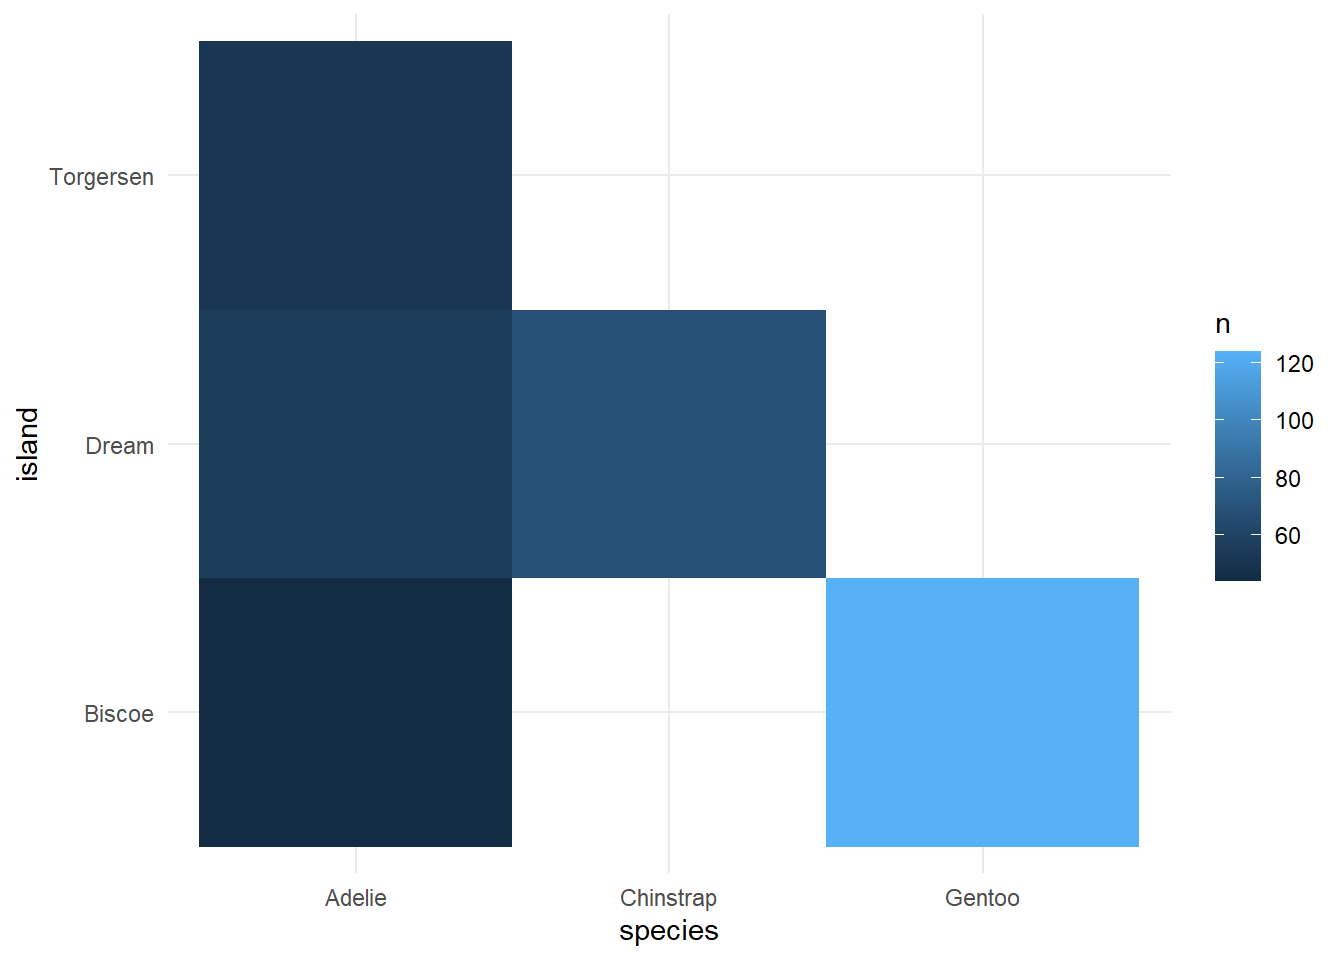
\includegraphics{DataExploration_files/figure-latex/unnamed-chunk-15-1.pdf}
What can we infer from the scatterplot?

What if we tried to group our plot by transmission? Do we learn anything
new?

\begin{Shaded}
\begin{Highlighting}[]
\NormalTok{usedcars }\OperatorTok
\StringTok{  }\KeywordTok{ggplot}\NormalTok{() }\OperatorTok{+}
\StringTok{  }\KeywordTok{geom_point}\NormalTok{(}\DataTypeTok{mapping =} \KeywordTok{aes}\NormalTok{(}\DataTypeTok{x =}\NormalTok{ mileage, }\DataTypeTok{y =}\NormalTok{ price, }\DataTypeTok{color =}\NormalTok{ transmission)) }\OperatorTok{+}
\StringTok{  }\KeywordTok{labs}\NormalTok{(}\DataTypeTok{title =} \StringTok{"Scatterplot of Price vs. Mileage"}\NormalTok{, }\DataTypeTok{x =} \StringTok{"Used Car Odometer (mi.)"}\NormalTok{, }\DataTypeTok{y =} \StringTok{"Used Car Price ($)"}\NormalTok{)}
\end{Highlighting}
\end{Shaded}

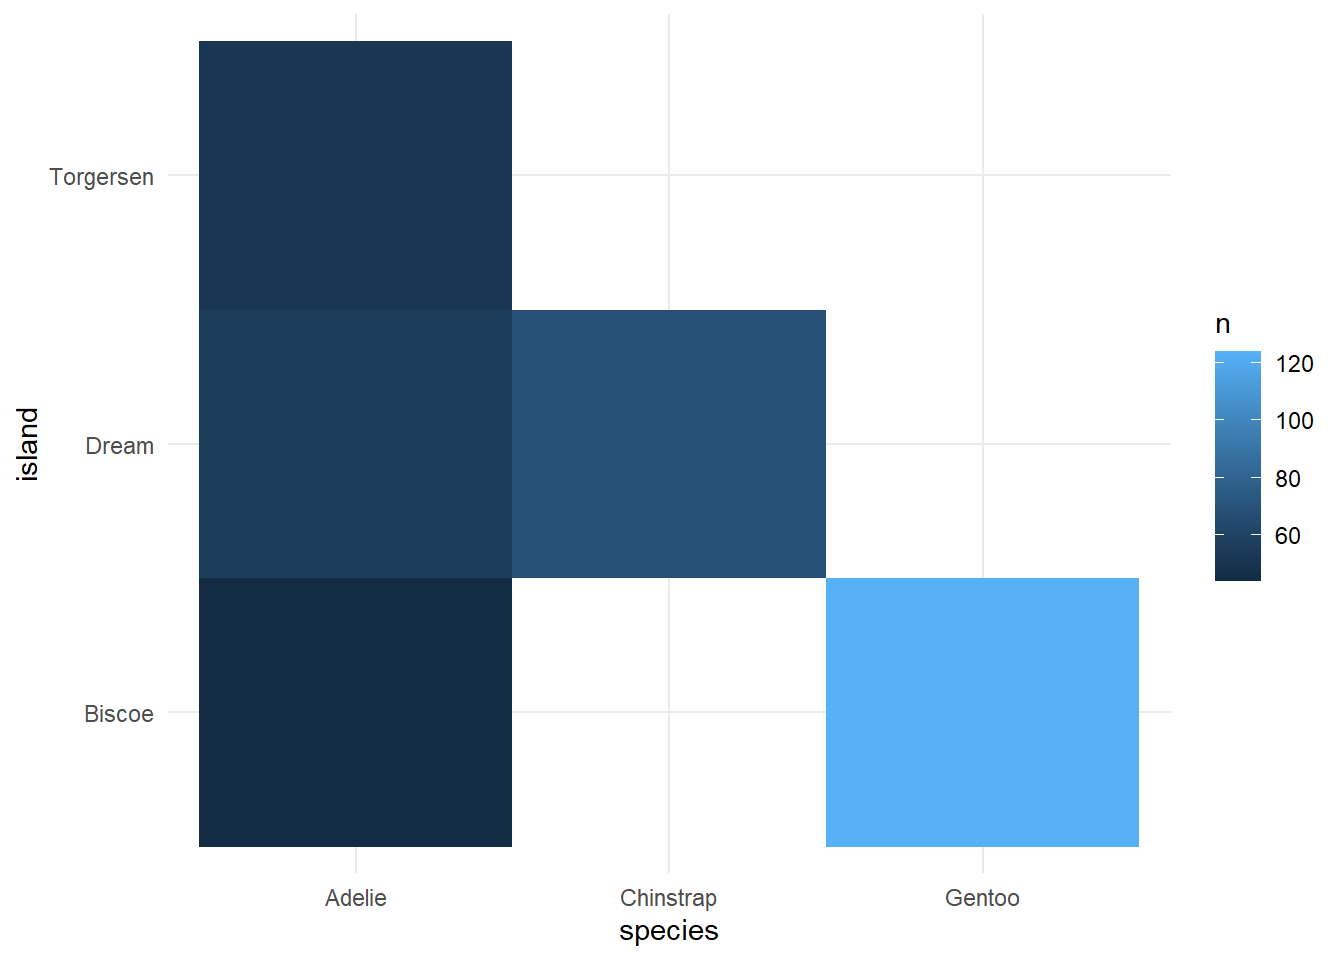
\includegraphics{DataExploration_files/figure-latex/unnamed-chunk-16-1.pdf}

What about grouping by model?

\begin{Shaded}
\begin{Highlighting}[]
\NormalTok{usedcars }\OperatorTok
\StringTok{  }\KeywordTok{ggplot}\NormalTok{() }\OperatorTok{+}
\StringTok{  }\KeywordTok{geom_point}\NormalTok{(}\DataTypeTok{mapping =} \KeywordTok{aes}\NormalTok{(}\DataTypeTok{x =}\NormalTok{ mileage, }\DataTypeTok{y =}\NormalTok{ price, }\DataTypeTok{color =}\NormalTok{ model)) }\OperatorTok{+}
\StringTok{  }\KeywordTok{labs}\NormalTok{(}\DataTypeTok{title =} \StringTok{"Scatterplot of Price vs. Mileage"}\NormalTok{, }\DataTypeTok{x =} \StringTok{"Used Car Odometer (mi.)"}\NormalTok{, }\DataTypeTok{y =} \StringTok{"Used Car Price ($)"}\NormalTok{)}
\end{Highlighting}
\end{Shaded}

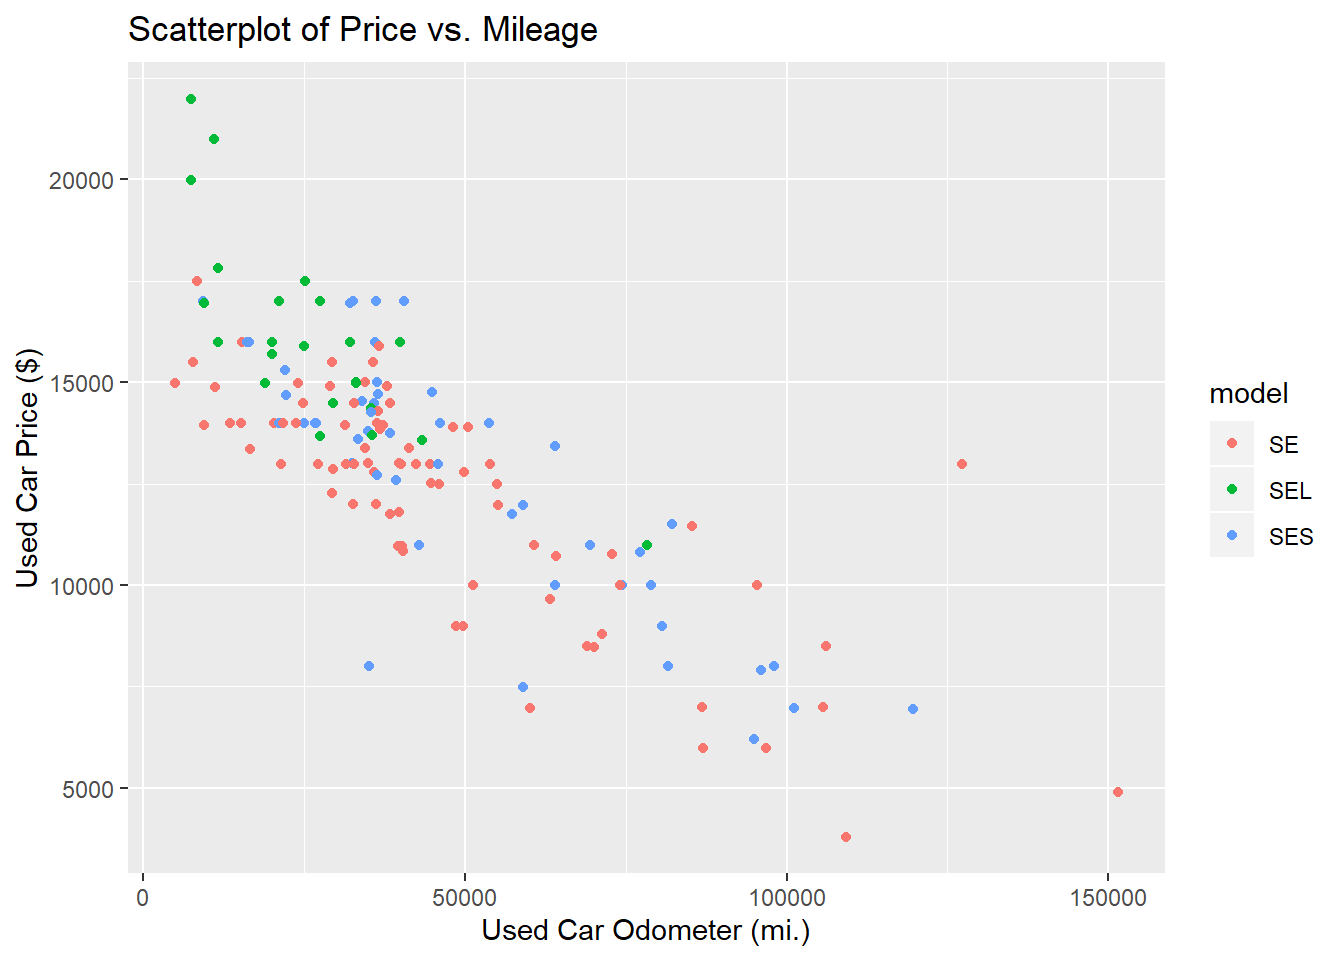
\includegraphics{DataExploration_files/figure-latex/unnamed-chunk-17-1.pdf}

And when you group by year, what do we see?

\begin{Shaded}
\begin{Highlighting}[]
\NormalTok{usedcars }\OperatorTok
\StringTok{  }\KeywordTok{ggplot}\NormalTok{() }\OperatorTok{+}
\StringTok{  }\KeywordTok{geom_point}\NormalTok{(}\DataTypeTok{mapping =} \KeywordTok{aes}\NormalTok{(}\DataTypeTok{x =}\NormalTok{ mileage, }\DataTypeTok{y =}\NormalTok{ price, }\DataTypeTok{color =}\NormalTok{ year)) }\OperatorTok{+}
\StringTok{  }\KeywordTok{labs}\NormalTok{(}\DataTypeTok{title =} \StringTok{"Scatterplot of Price vs. Mileage"}\NormalTok{, }\DataTypeTok{x =} \StringTok{"Used Car Odometer (mi.)"}\NormalTok{, }\DataTypeTok{y =} \StringTok{"Used Car Price ($)"}\NormalTok{)}
\end{Highlighting}
\end{Shaded}

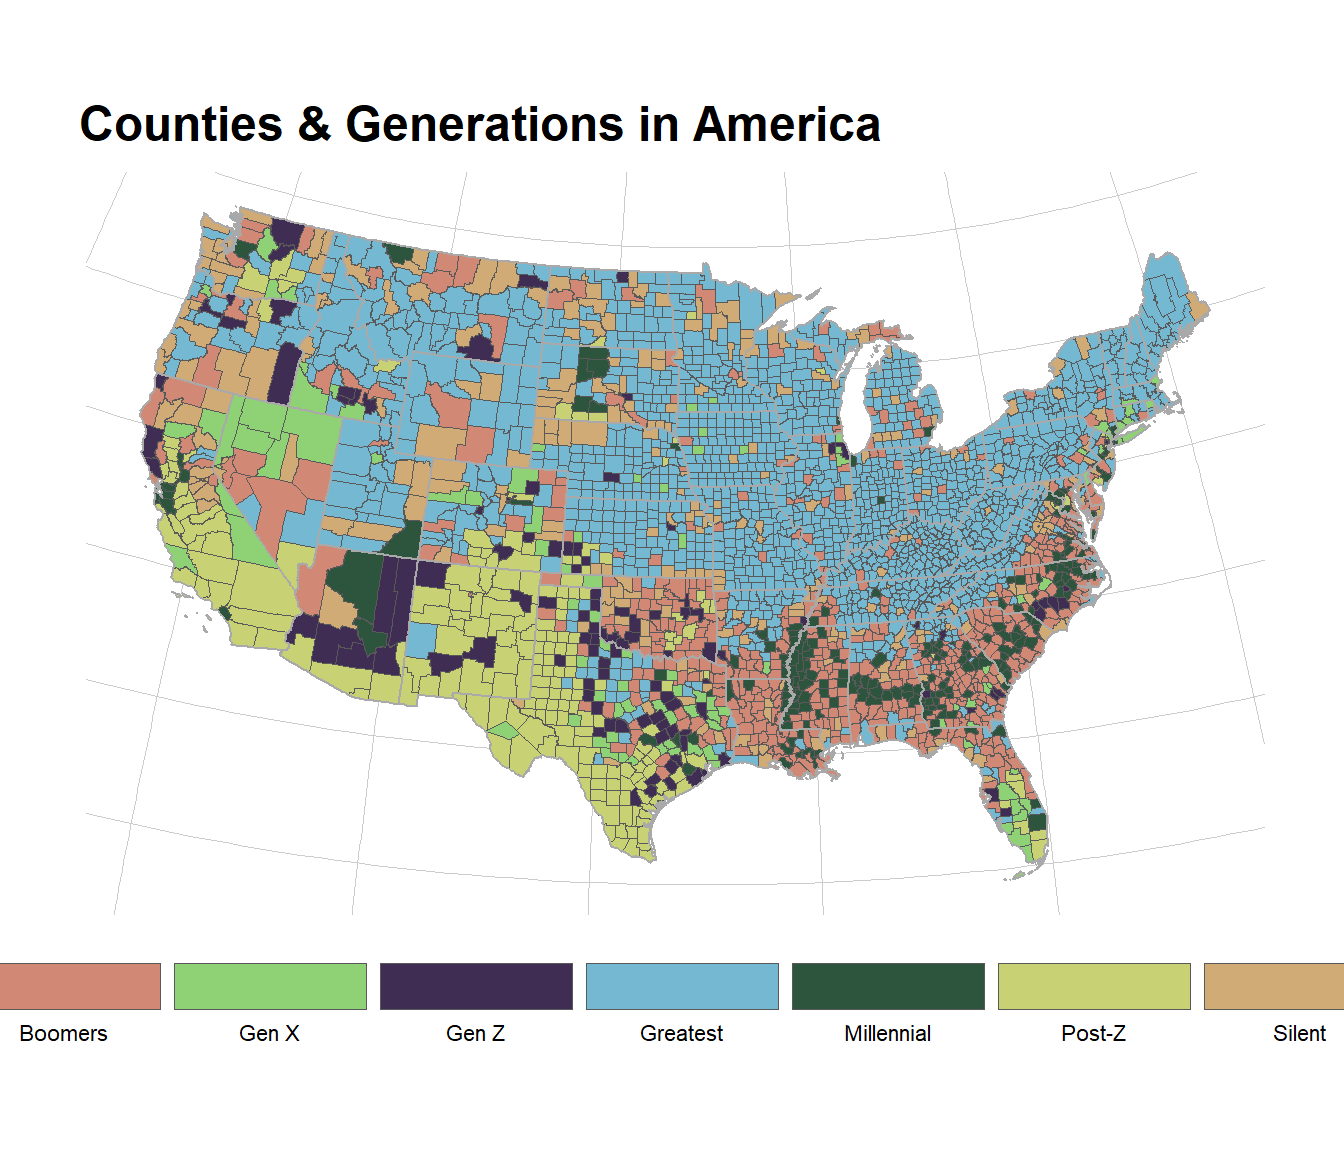
\includegraphics{DataExploration_files/figure-latex/unnamed-chunk-18-1.pdf}

Using a box plot to show price by year reveals the expected.

\begin{Shaded}
\begin{Highlighting}[]
\NormalTok{usedcars }\OperatorTok
\StringTok{  }\KeywordTok{ggplot}\NormalTok{() }\OperatorTok{+}
\StringTok{  }\KeywordTok{geom_boxplot}\NormalTok{(}\DataTypeTok{mapping =} \KeywordTok{aes}\NormalTok{(}\DataTypeTok{x =}\NormalTok{ year, }\DataTypeTok{y =}\NormalTok{ price, }\DataTypeTok{fill =}\NormalTok{ year)) }\OperatorTok{+}
\StringTok{  }\KeywordTok{labs}\NormalTok{(}\DataTypeTok{title =} \StringTok{"Boxplot of Used Car Prices by Year"}\NormalTok{, }\DataTypeTok{x =} \StringTok{"Year"}\NormalTok{, }\DataTypeTok{y =} \StringTok{"Price ($)"}\NormalTok{)}
\end{Highlighting}
\end{Shaded}

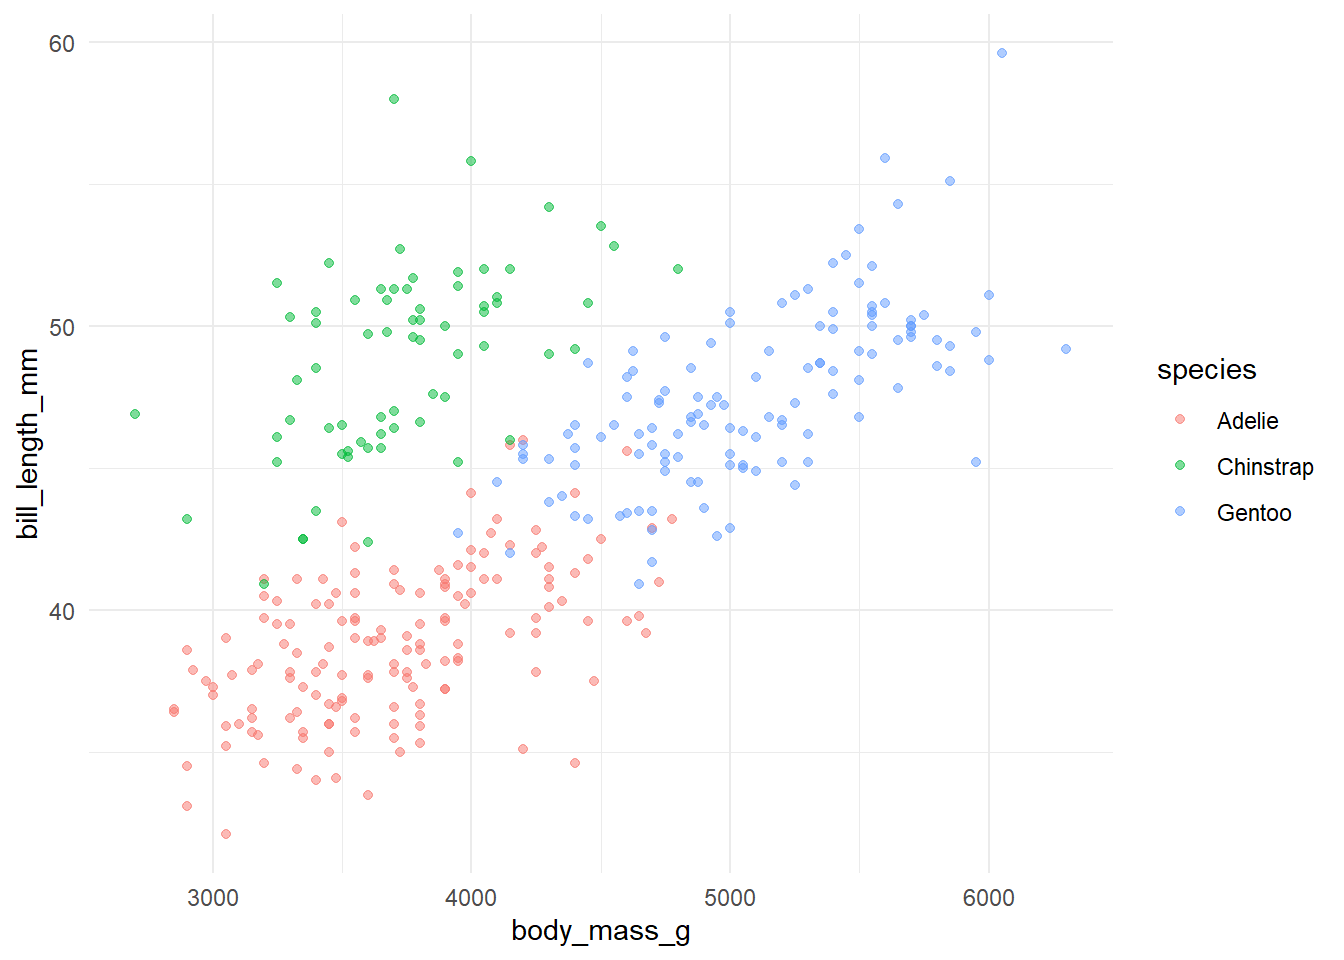
\includegraphics{DataExploration_files/figure-latex/unnamed-chunk-19-1.pdf}

What does the boxplot of price by model type tell us?

\begin{Shaded}
\begin{Highlighting}[]
\NormalTok{usedcars }\OperatorTok
\StringTok{  }\KeywordTok{ggplot}\NormalTok{() }\OperatorTok{+}
\StringTok{  }\KeywordTok{geom_boxplot}\NormalTok{(}\DataTypeTok{mapping =} \KeywordTok{aes}\NormalTok{(}\DataTypeTok{x =}\NormalTok{ model, }\DataTypeTok{y =}\NormalTok{ price, }\DataTypeTok{fill =}\NormalTok{ model)) }\OperatorTok{+}
\StringTok{  }\KeywordTok{labs}\NormalTok{(}\DataTypeTok{title =} \StringTok{"Boxplot of Used Car Prices by Model"}\NormalTok{, }\DataTypeTok{x =} \StringTok{"Model"}\NormalTok{, }\DataTypeTok{y =} \StringTok{"Price ($)"}\NormalTok{)}
\end{Highlighting}
\end{Shaded}

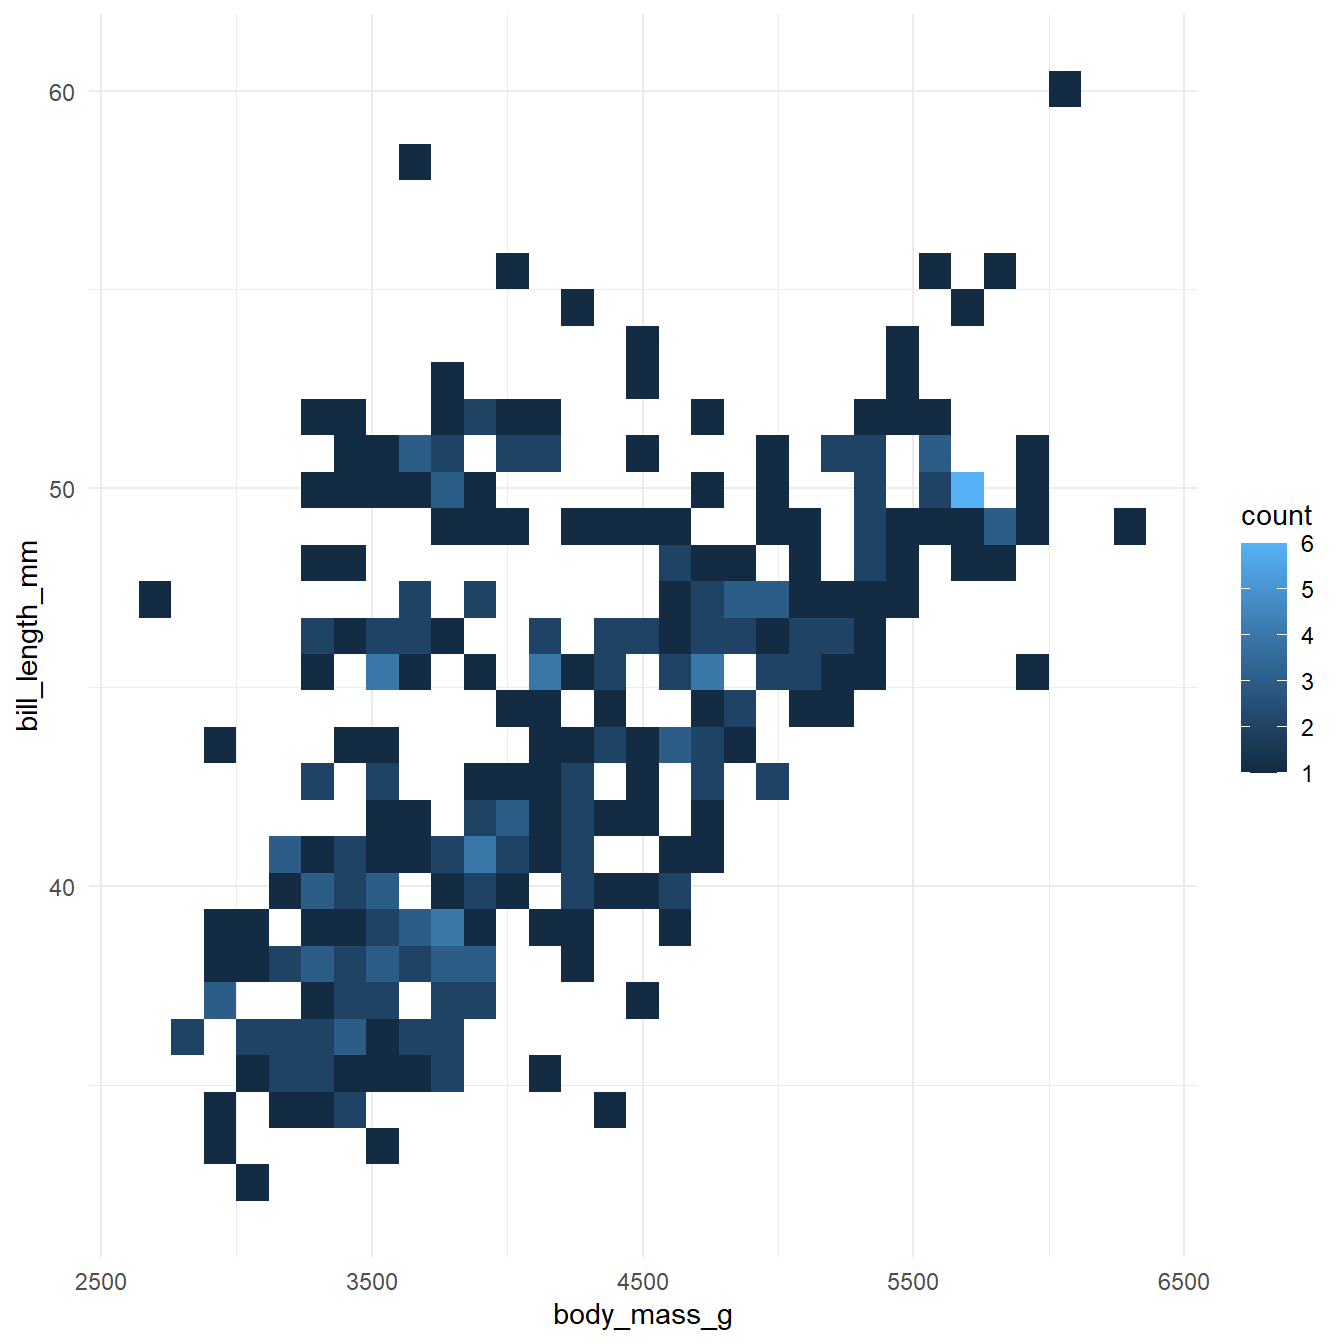
\includegraphics{DataExploration_files/figure-latex/unnamed-chunk-20-1.pdf}

\$Net Interest Margin =
\frac{(Investment Returns - Interest Expense)}{Average Earning Assets}
\$


\end{document}
